\section{Wöhrner Wöör (WöWö)}

\subsection{Overview and Digital Evolution}

The \emph{Wöhrner Wöör} is a Low German dictionary from the Dithmarschen region (North Low Saxon), compiled by Peter Neuber (born 1939 in Szczecin), a linguist and educator. The dictionary was created with the goal of documenting and preserving the traditional vocabulary and expressions of Plattdeutsch while simultaneously adapting the language to modern contexts. Beyond recording historical terms, Neuber sought to introduce neologisms for contemporary concepts that previously lacked Low German equivalents, integrating them into the lexicon.

First published in 2001 in Wöhrden, the \emph{Wöhrner Wöör} consists of 699 pages and serves as a German-to-Low-German reference work specific to the Dithmarschen dialect (Fig. \ref{fig-woewoe-excerpt}). Following its initial print release, the dictionary has undergone continuous expansion, with subsequent versions distributed exclusively in digital formats such as Microsoft Word and PDF. %Within the \emph{Niederdeutsche Literaturdatenbank} (Low German Literature Database), the 2017 Word edition is the most frequently cited version. %% more of an DWN artifact
The latest version, titled \emph{Ditschiplatt: Wöhrner Wöör} from January 2019 is accessible online.\footnote{\url{https://ditschiplatt.de/woehrner-woeoer/}}

% this is relevant, but we need to get below 12 pages
\ign{
    A major structural update took place at the end of 2015, when Neuber transitioned the dictionary's orthography to an extended version of the SASS spelling system, originally developed by Johannes Sass, to incorporate diacritical marks (macrons) to denote diphthongs, thereby enhancing phonological precision. Beyond its lexical entries, the dictionary includes a comprehensive user guide for navigating the digital version in MS Office (Word), as well as pronunciation information and a grammatical overview of the Dithmarschen dialect, with a particular focus on verbs, nouns, and adjectives.
}

Despite a remarkable level of detail and complex structure, %its detailed documentation and modern adaptation efforts, 
the \emph{Wöhrner Wöör} remains primarily a resource for human readers, lacking structured machine-readable representations that would facilitate its use in NLP applications. Thus, our goal was to convert the \emph{Wöhrner Wöör} into an RDF-based format following the OntoLex-Lemon model to ensure interoperability with other lexical datasets and enable the dictionary’s inclusion in the LLOD cloud, paving the way for broader computational applications and cross-linguistic research.

\ign{
    \begin{figure}
        \centering
        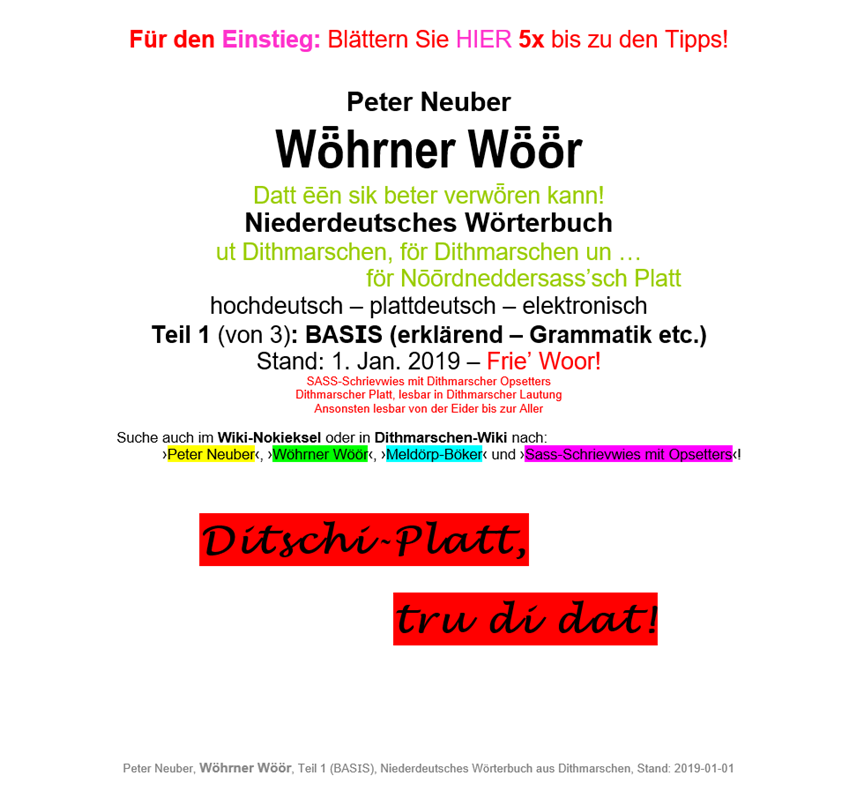
\includegraphics[width=1\linewidth]{img/woewoe_cover.png}
        \caption{Front page of the \emph{Wöörner Wöhr} dictionary in docx format.}
        \label{fig-woewoe-front}
    \end{figure}
}
    
\begin{figure*}
    \centering
    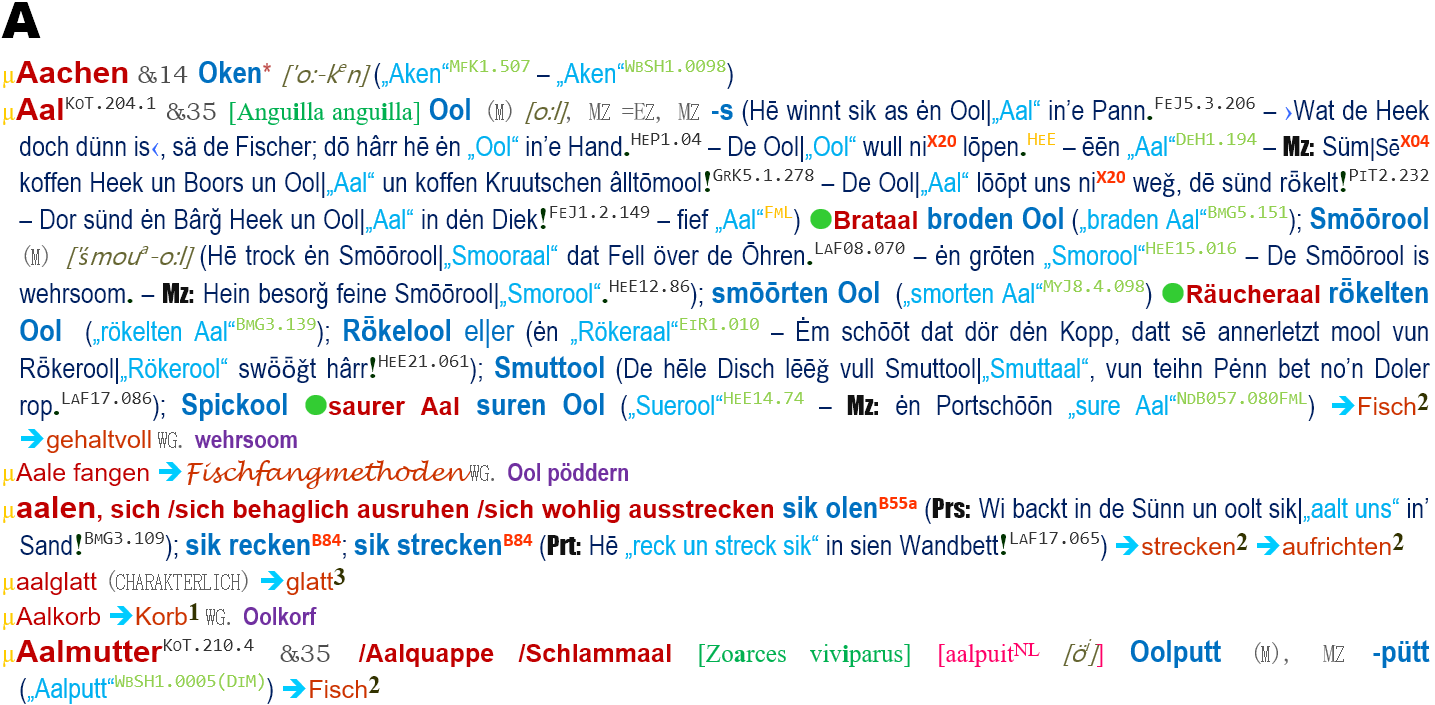
\includegraphics[width=0.95\linewidth]{img/woewoe_excerpt-hires.png}
    \caption{Excerpt of the first entries under ‘A’ from the beginning of the lexical part of the \emph{Wöörner Wöhr} dictionary in docx format.}
    \label{fig-woewoe-excerpt}
\end{figure*}

\subsection{Converting the WöWö}

Converting the \emph{Wöhrner Wöör} into an MRD posed a significant challenge due to its highly fragmented DOCX format. The extensive use of diverse fonts, colors, and sizes—each encoding different functions—meant that the underlying text information was split into numerous small fragments within the Office Open XML format. This complexity required a multi-stage processing pipeline via Python for extraction, merging, and transformation of the text information:

\begin{enumerate}
    \item {\textbf{Extracting relevant data from XML}}\\  
    First, the verbose XML structure of the Word document is parsed using Python’s \texttt{xml.etree}. Each text run (\texttt{<w:r>}) is extracted along with its formatting metadata (font, color, and size), leveraging XML namespaces to accurately retrieve \texttt{<w:t>} (text) and \texttt{<w:rPr>} (formatting) elements. This step generates a preliminary \texttt{DataFrame} stored as a raw CSV file.

    \item {\textbf{Merging Consecutive Text Blocks}}\\  
   Due to fragmentation, consecutive text blocks with identical formatting are merged. A Python script iterates through the DataFrame, combining segments that share the same color and size. This merging produces a more coherent CSV that better reflects the original document’s logical layout.

    \item {\textbf{Structuring the Data into a Lexical CSV}}\\  
    With the merged text available, the next step involves classifying and extracting entries into five columns, depending on the corresponding formatting:
    \begin{enumerate}
        \item {\textbf{High German Main Lemma}}
        \item {\textbf{High German Sublemma}}\\Potential subentries per lexical entry.
        \item {\textbf{Low German Translation}}
        \item {\textbf{Low German Additions}}\\ Additional grammatical information -- mainly plural forms -- that has the same formatting as the corresponding Low German lexical entry.
        \item {\textbf{Low German IPA Information}}\\Low German phonetic transcriptions.
    \end{enumerate}
    This structured CSV serves as the foundation for converting the data into RDF.

    \item {\textbf{Generating RDF (Turtle Format)}}\\ 
    Separate Python scripts convert the structured CSV data into RDF (Turtle):
    \begin{enumerate}
        \item {\textbf{High German Entries:}} Entries are first grouped by main lemmas. The script converts them into \texttt{ontolex:LexicalEntry} nodes, each with its own \texttt{ontolex:LexicalSense}. Additional information, such as synonymous terms or usage examples -- but mostly plural information or alternative spellings (e.g., variations in single vowels) -- is included as \texttt{ontolex:otherForm}. In the case of alternative spellings or plural information, these additions are usually not full words but only the modifications, such as the suffix '-s'. 
        
        A custom property \texttt{subEntry} links to related sublemmas. For all existing sublemmas, individual lexical entries with their own lexical senses are generated in a similar way.
        \item {\textbf{Low German Translations:}} The Low German translations are processed into lexical entries, each with its own lexical sense. If available, IPA notation is incorporated into the canonical form as \texttt{ontolex:phoneticRep}.
        \item {\textbf{Linking Translations:}} Finally, unique \texttt{vartrans:Translation} entries are generated to link source senses (High German main or sublemmas) with their corresponding target senses (Low German translations).
    \end{enumerate}

    \item {\textbf{Post-Processing}}\\  
    The generated Turtle files are further refined using a regex-based clean-up. This post-processing step removes unnecessary whitespaces, replaces dashes with underscores, and normalizes punctuation to ensure that the RDF output adheres to the required naming conventions and syntactic standards.
\end{enumerate}

\begin{figure*}
    \centering
    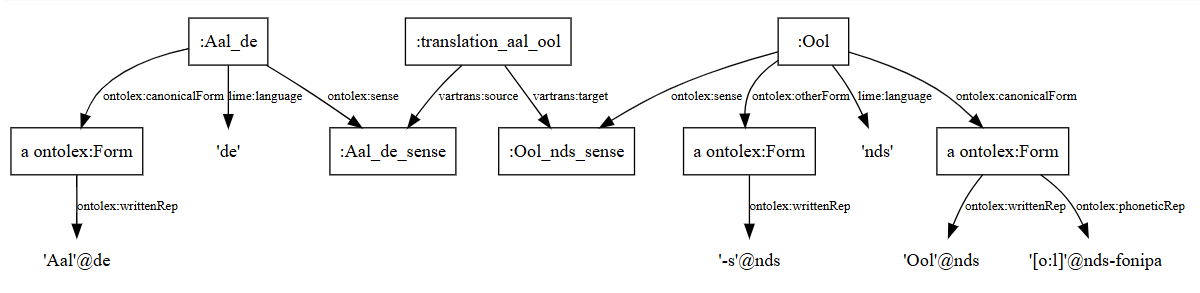
\includegraphics[width=1.0\linewidth]{aal-rdf-graph.png}
    \caption{Resulting RDF graph for the entry \word{Aal} `eal'.}
    \label{fig:aal-graph}
\end{figure*}

\noindent
This comprehensive pipeline successfully transforms the fragmented DOCX format of the \emph{Wöhrner Wöör} into a coherent RDF dataset (cf. Fig. \ref{fig:aal-graph}), aligning the dictionary with the Ontolex-Lemon model, and thus builds a baseline for LLOD integration. So far, this extraction process has focused on retrieving the most essential information -- lexical entries, written and phonetic representations, and their corresponding translations. However, the \emph{Wöhrner Wöör} contains numerous additional details for each entry, such as references and usage examples, which are more challenging to extract due to the complexity of the fragmented format.



%CF: this was a vertical alternative. However still too small for a single column.
%\begin{figure*}
%    \centering
%    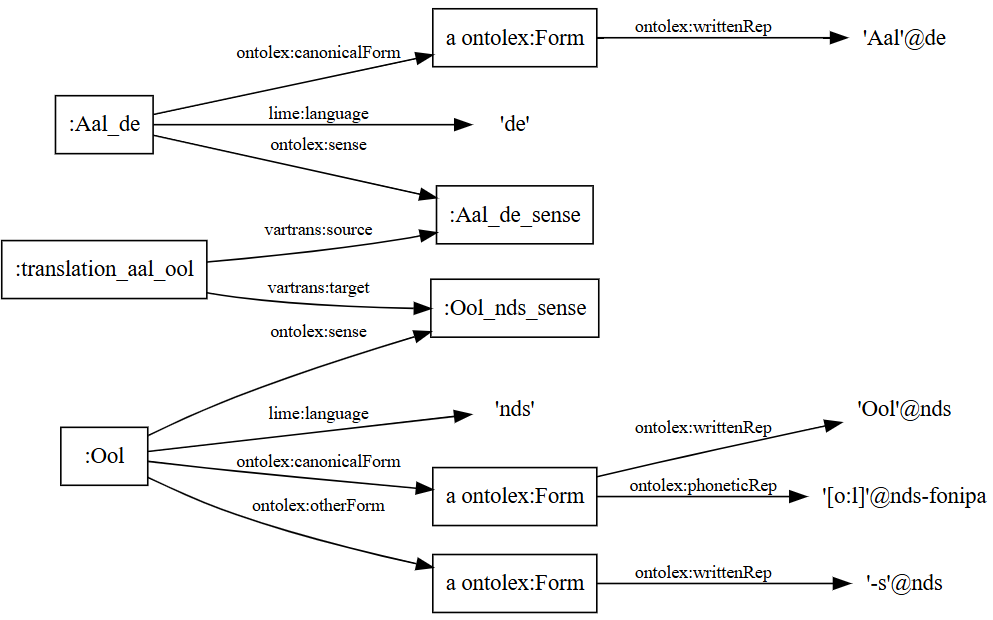
\includegraphics[width=0.6\linewidth]{woewoe-entry-eel.png}
%    \caption{Enter Caption}
%    \label{fig:enter-label}
%\end{figure*}


%digraph finite_state_machine {
%    rankdir=UD;
%    size="8,5"
%    node [shape=box, fontname="CMU Serif"];
%        edge [fontname="CMU Serif", fontsize=11];
%
%        Aal [label=":Aal_de"];
%        Aal_canonicalForm [label="a ontolex:Form"];
%        Aal_sense [label=":Aal_de_sense"];
%        translation_aal_ool [label=":translation_aal_ool"];
%        Ool [label=":Ool"];
%        Ool_canonicalForm [label="a ontolex:Form"];
%        Ool_sense [label=":Ool_nds_sense"];
%        Ool_otherForm [label="a ontolex:Form"];
%
%        Aal -> "'de'" [label = "lime:language"];
%        Aal -> Aal_canonicalForm [label = "ontolex:canonicalForm"];
%        Aal -> Aal_sense [label = "ontolex:sense"];
%        translation_aal_ool -> Aal_sense [label = "vartrans:source"];
%        translation_aal_ool -> Ool_sense [label = "vartrans:target"];
%        Ool -> Ool_canonicalForm [label = "ontolex:canonicalForm"];
%        Ool -> Ool_sense [label = "ontolex:sense"];
%        Ool -> Ool_otherForm [label = "ontolex:otherForm"];
%        Ool -> "'nds'" [label = "lime:language"];
%        Aal_canonicalForm -> "'Aal'@de" [label = "ontolex:writtenRep"];
%        Ool_canonicalForm -> "'Ool'@nds" [label = "ontolex:writtenRep"];
%        Ool_canonicalForm -> "'[o:l]'@nds-fonipa" [label = "ontolex:phoneticRep"];
%        Ool_otherForm -> "'-s'@nds" [label = "ontolex:writtenRep"];
%
%        "'de'" [shape=none];
%        "'nds'" [shape=none];
%        "'Aal'@de" [shape=none];
%        "'Ool'@nds" [shape=none];
%        "'-s'@nds" [shape=none];
%        "'[o:l]'@nds-fonipa" [shape=none];
%}

